\chapter{Project 1: Blink}

\section{Overview}
This project is designed to provide a foundation for subsequent projects in this book (\textbf{and beyond}).
Over the course of this project, you will:
\begin{itemize}
    \item Create a simple circuit using your breadboard
    \item Write a program that runs in a loop
    \item Use MicroPython in your program to interact with your microcontroller's GPIO pins.
\end{itemize}
At the end of this project, your microcontroller should run a MicroPython program which alternates a
light between its ON and OFF states. Let's get started!
\begin{figure}[H]
\centering
    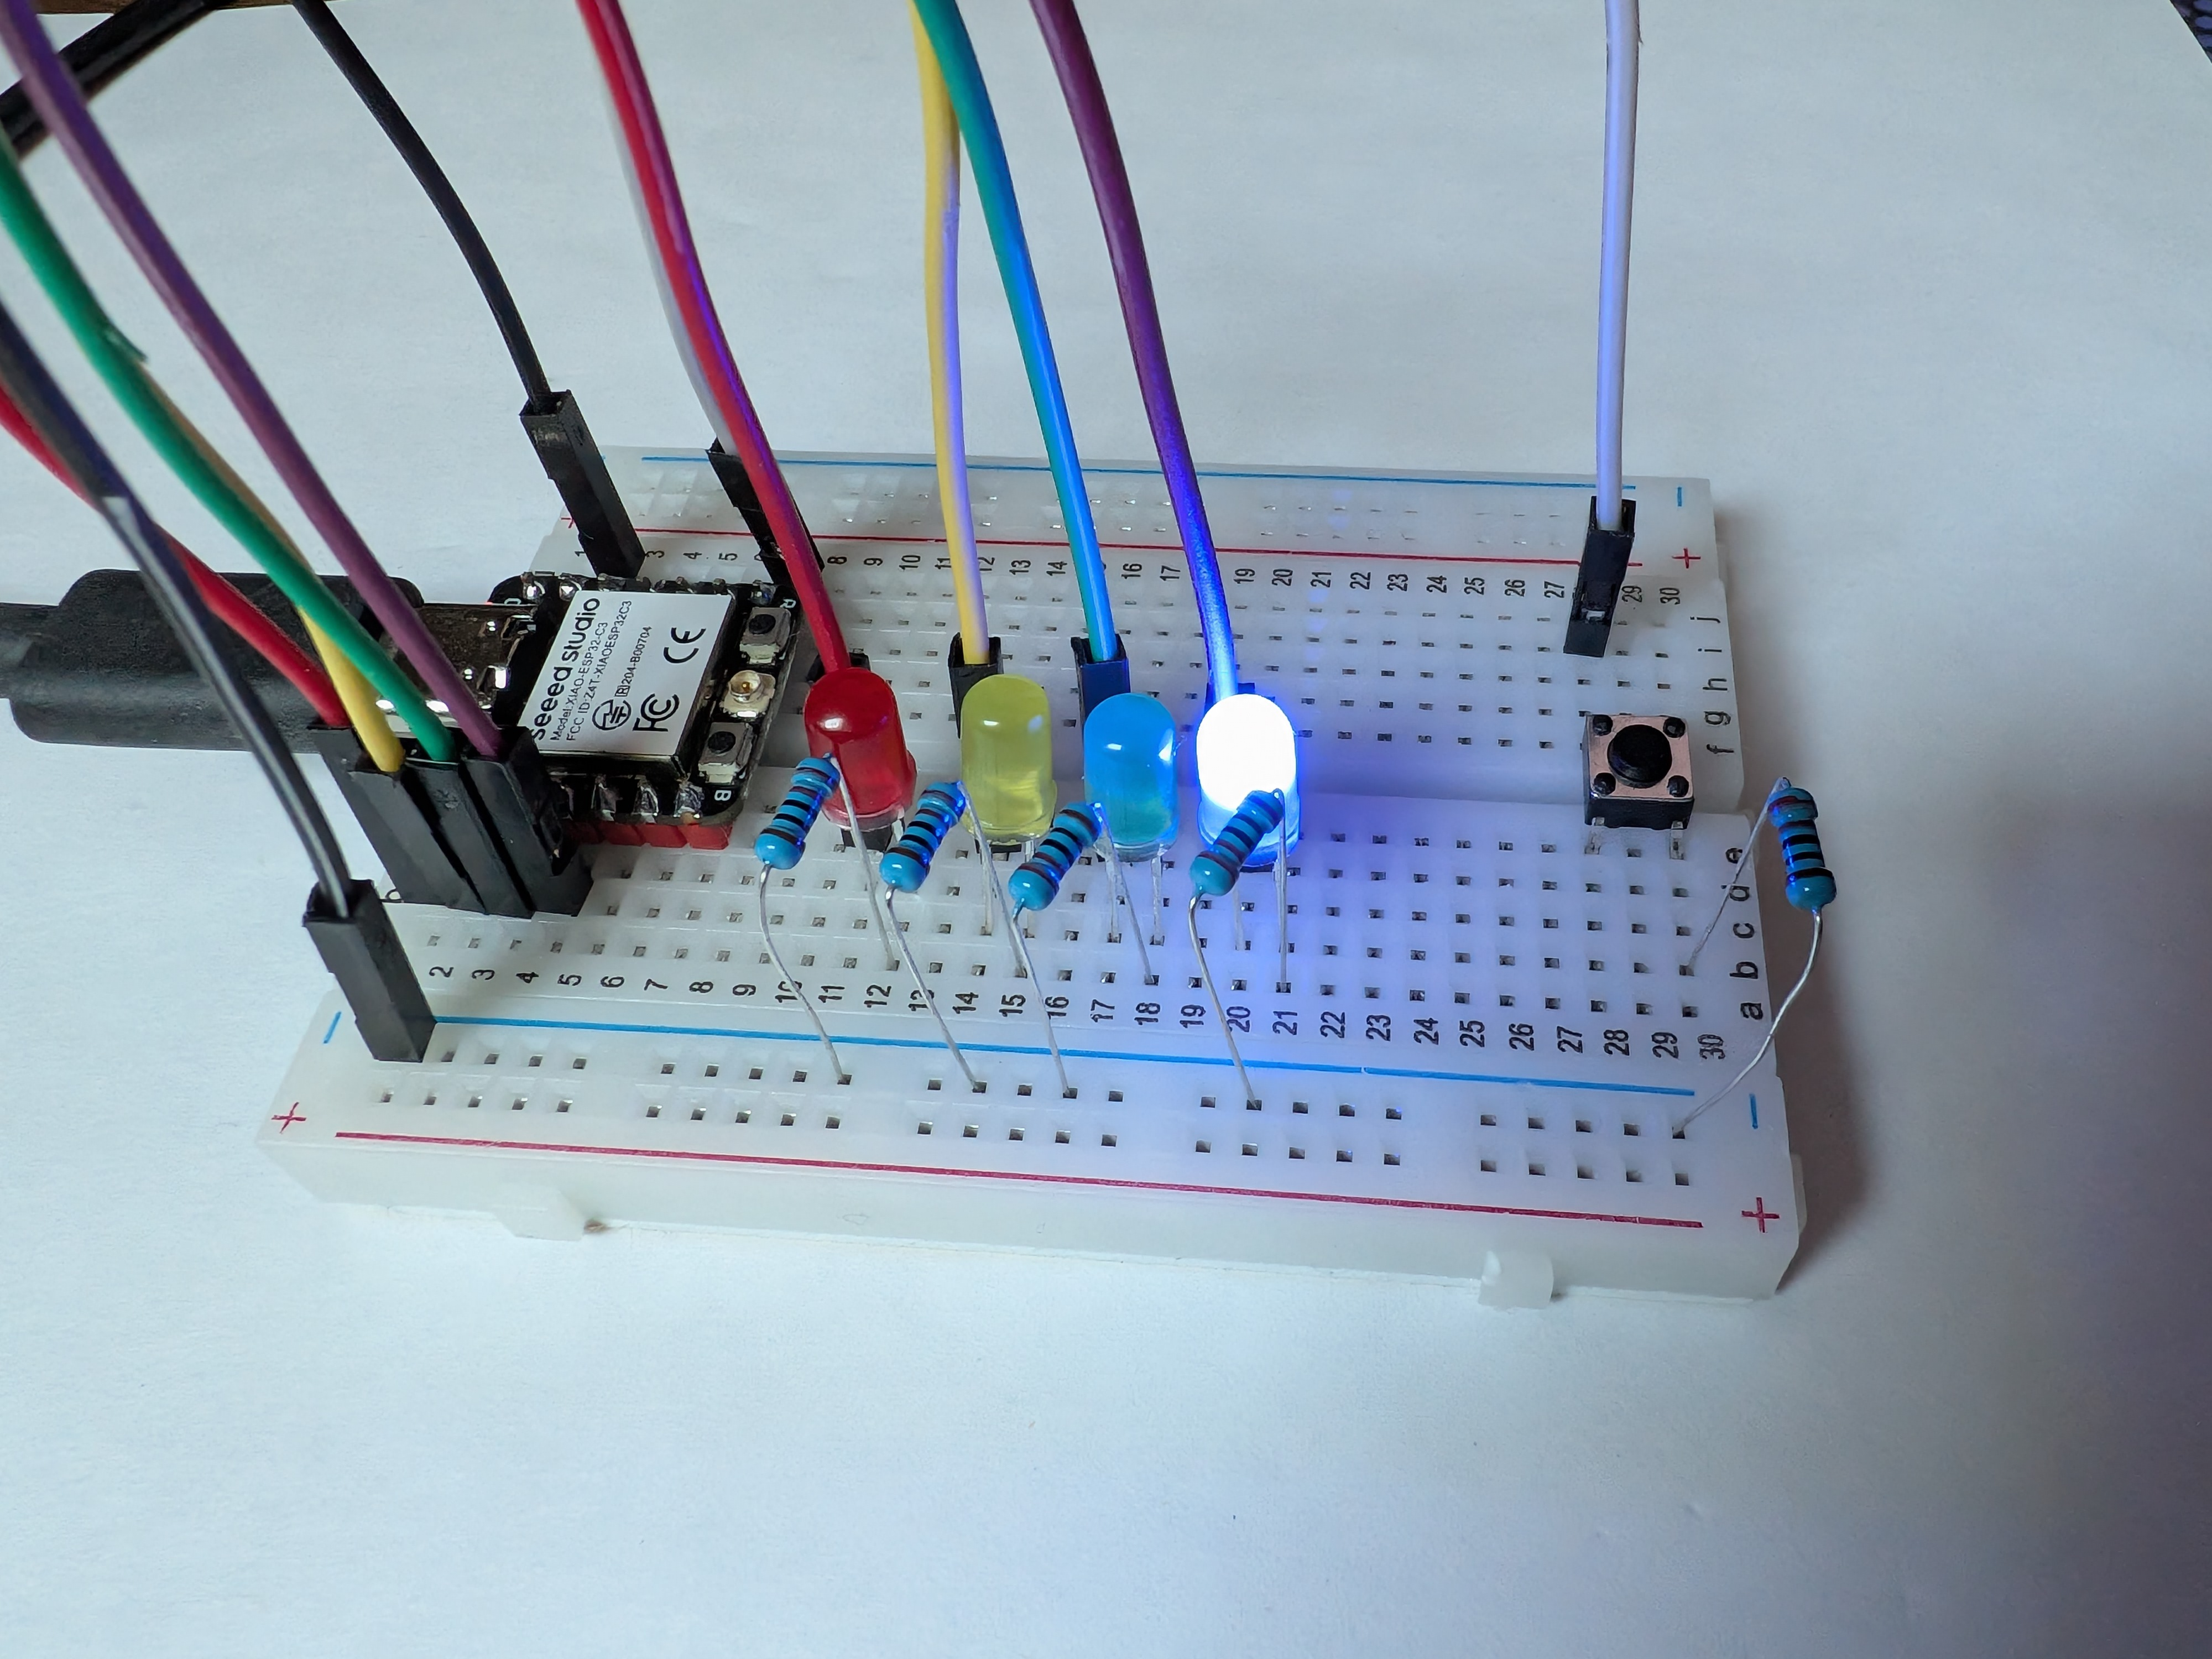
\includegraphics[width=.6\linewidth]{project_1/success!.jpg}
    \caption{The end result should look something like this}
\end{figure}

\pagebreak

\section{Directions}

\subsubsection{Remove previous components}
Before beginning, remove any components from prior chapters including LEDs, buttons, and wires. You may leave the
microcontroller attached to the breadboard.

\subsection{Creating the circuit}
Using jumper cables, you will be assembling a circuit between your microcontroller, your breadboard,
an LED, and a 220\si{\ohm} resistor.

\subsubsection{Attach the microcontroller to the breadboard}
Carefully insert the pins at the bottom of your microcontroller into the breadboard, making sure that the microcontroller is oriented such that:
\begin{itemize}
    \item The pin labeled \textbf{5V} is inserted in hole at \textbf{Column H, Row 1} of the breadboard (or \textbf{H1}, for short)
    \item The pin labeled \textbf{GPIO2} is inserted in hole \textbf{D1} of the breadboard
    \item The pin labeled \textbf{GPIO20} is inserted in hole \textbf{H7} of the breadboard
    \item the pin labeled \textbf{GPIO21} is inserted in hole \textbf{D7} of the breadboard
\end{itemize}
You may need to apply more pressure than expected to seat the microcontroller properly in the breadboard. When its over, it should look like this:

\begin{figure}[H]
    \centering
    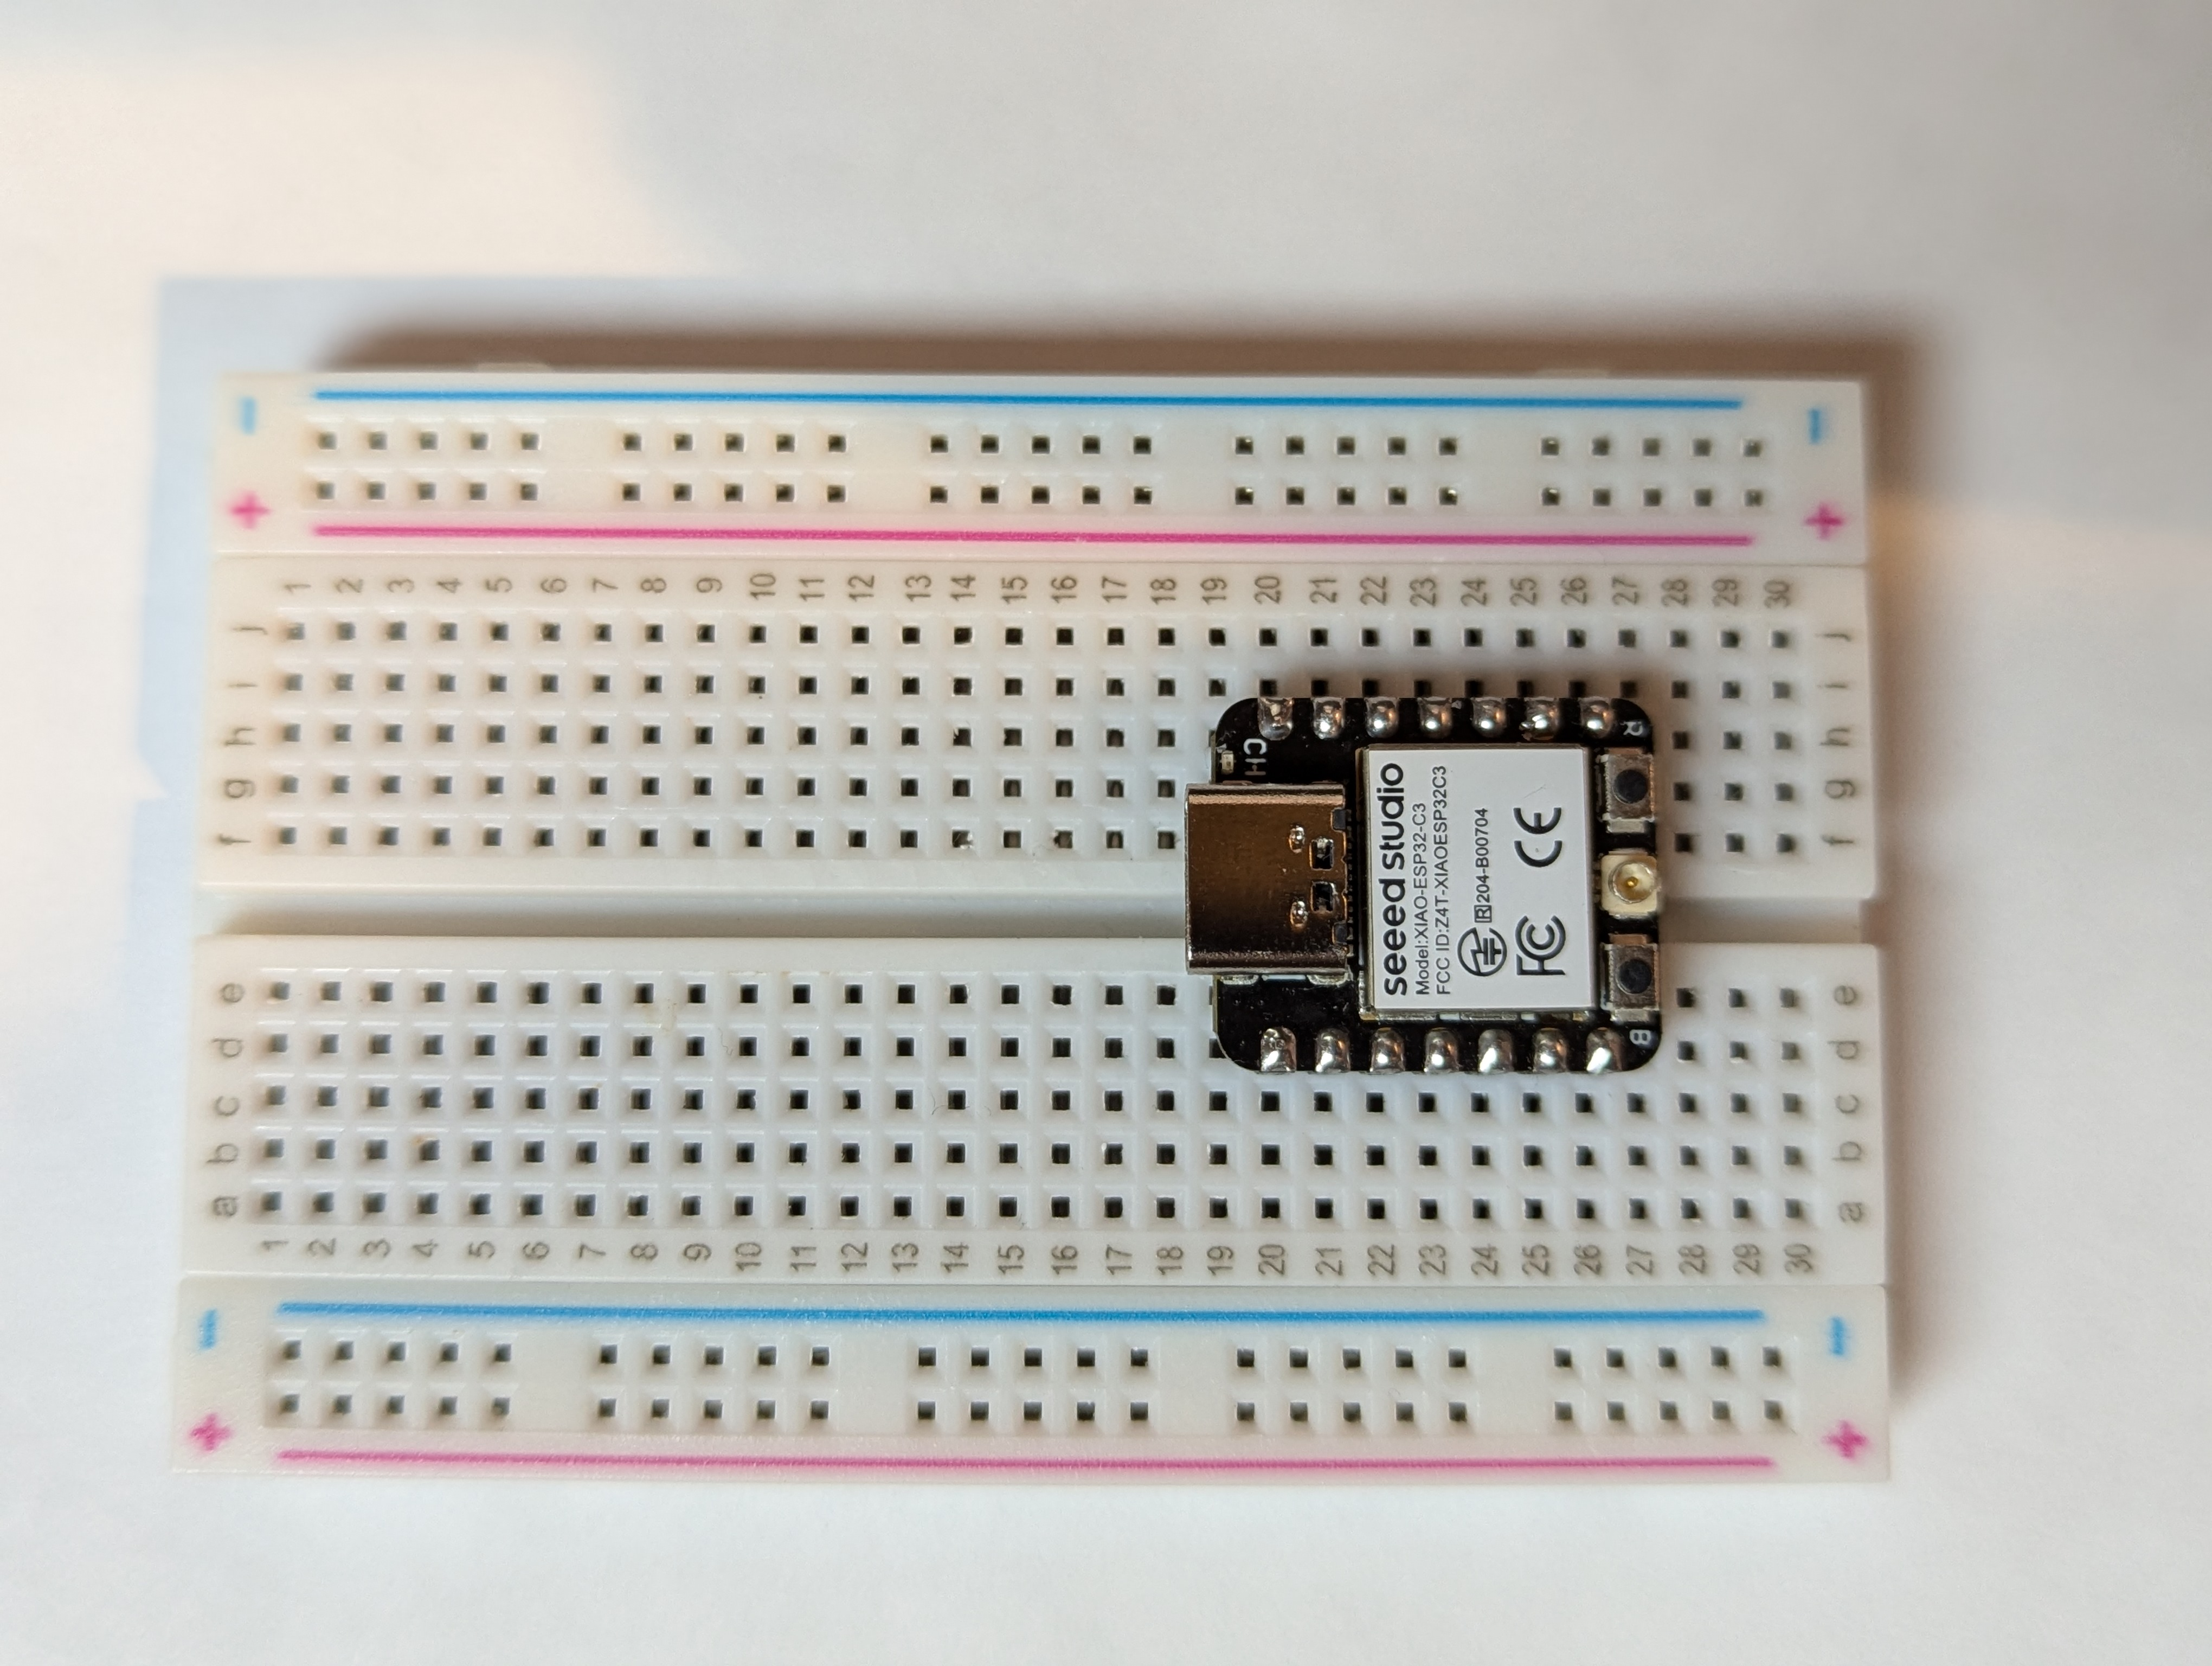
\includegraphics[width=.6\linewidth]{common/microcontroller_seated_in_breadboard.jpg}
    \caption{So far, so good!}
\end{figure}

\subsubsection{Connect the LED and Resistor}
Place an LED of your choice (the example image below uses RED) into the breadboard. The longer leg
should be placed in \textbf{B16} and the shorter leg should be placed in \textbf{B17}. Then place one
leg of a resistor (doesn't matter which one) in \textbf{A17} and the other in \textbf{A21}.

You should be left with something that looks like this:
\begin{figure}[H]
    \centering
    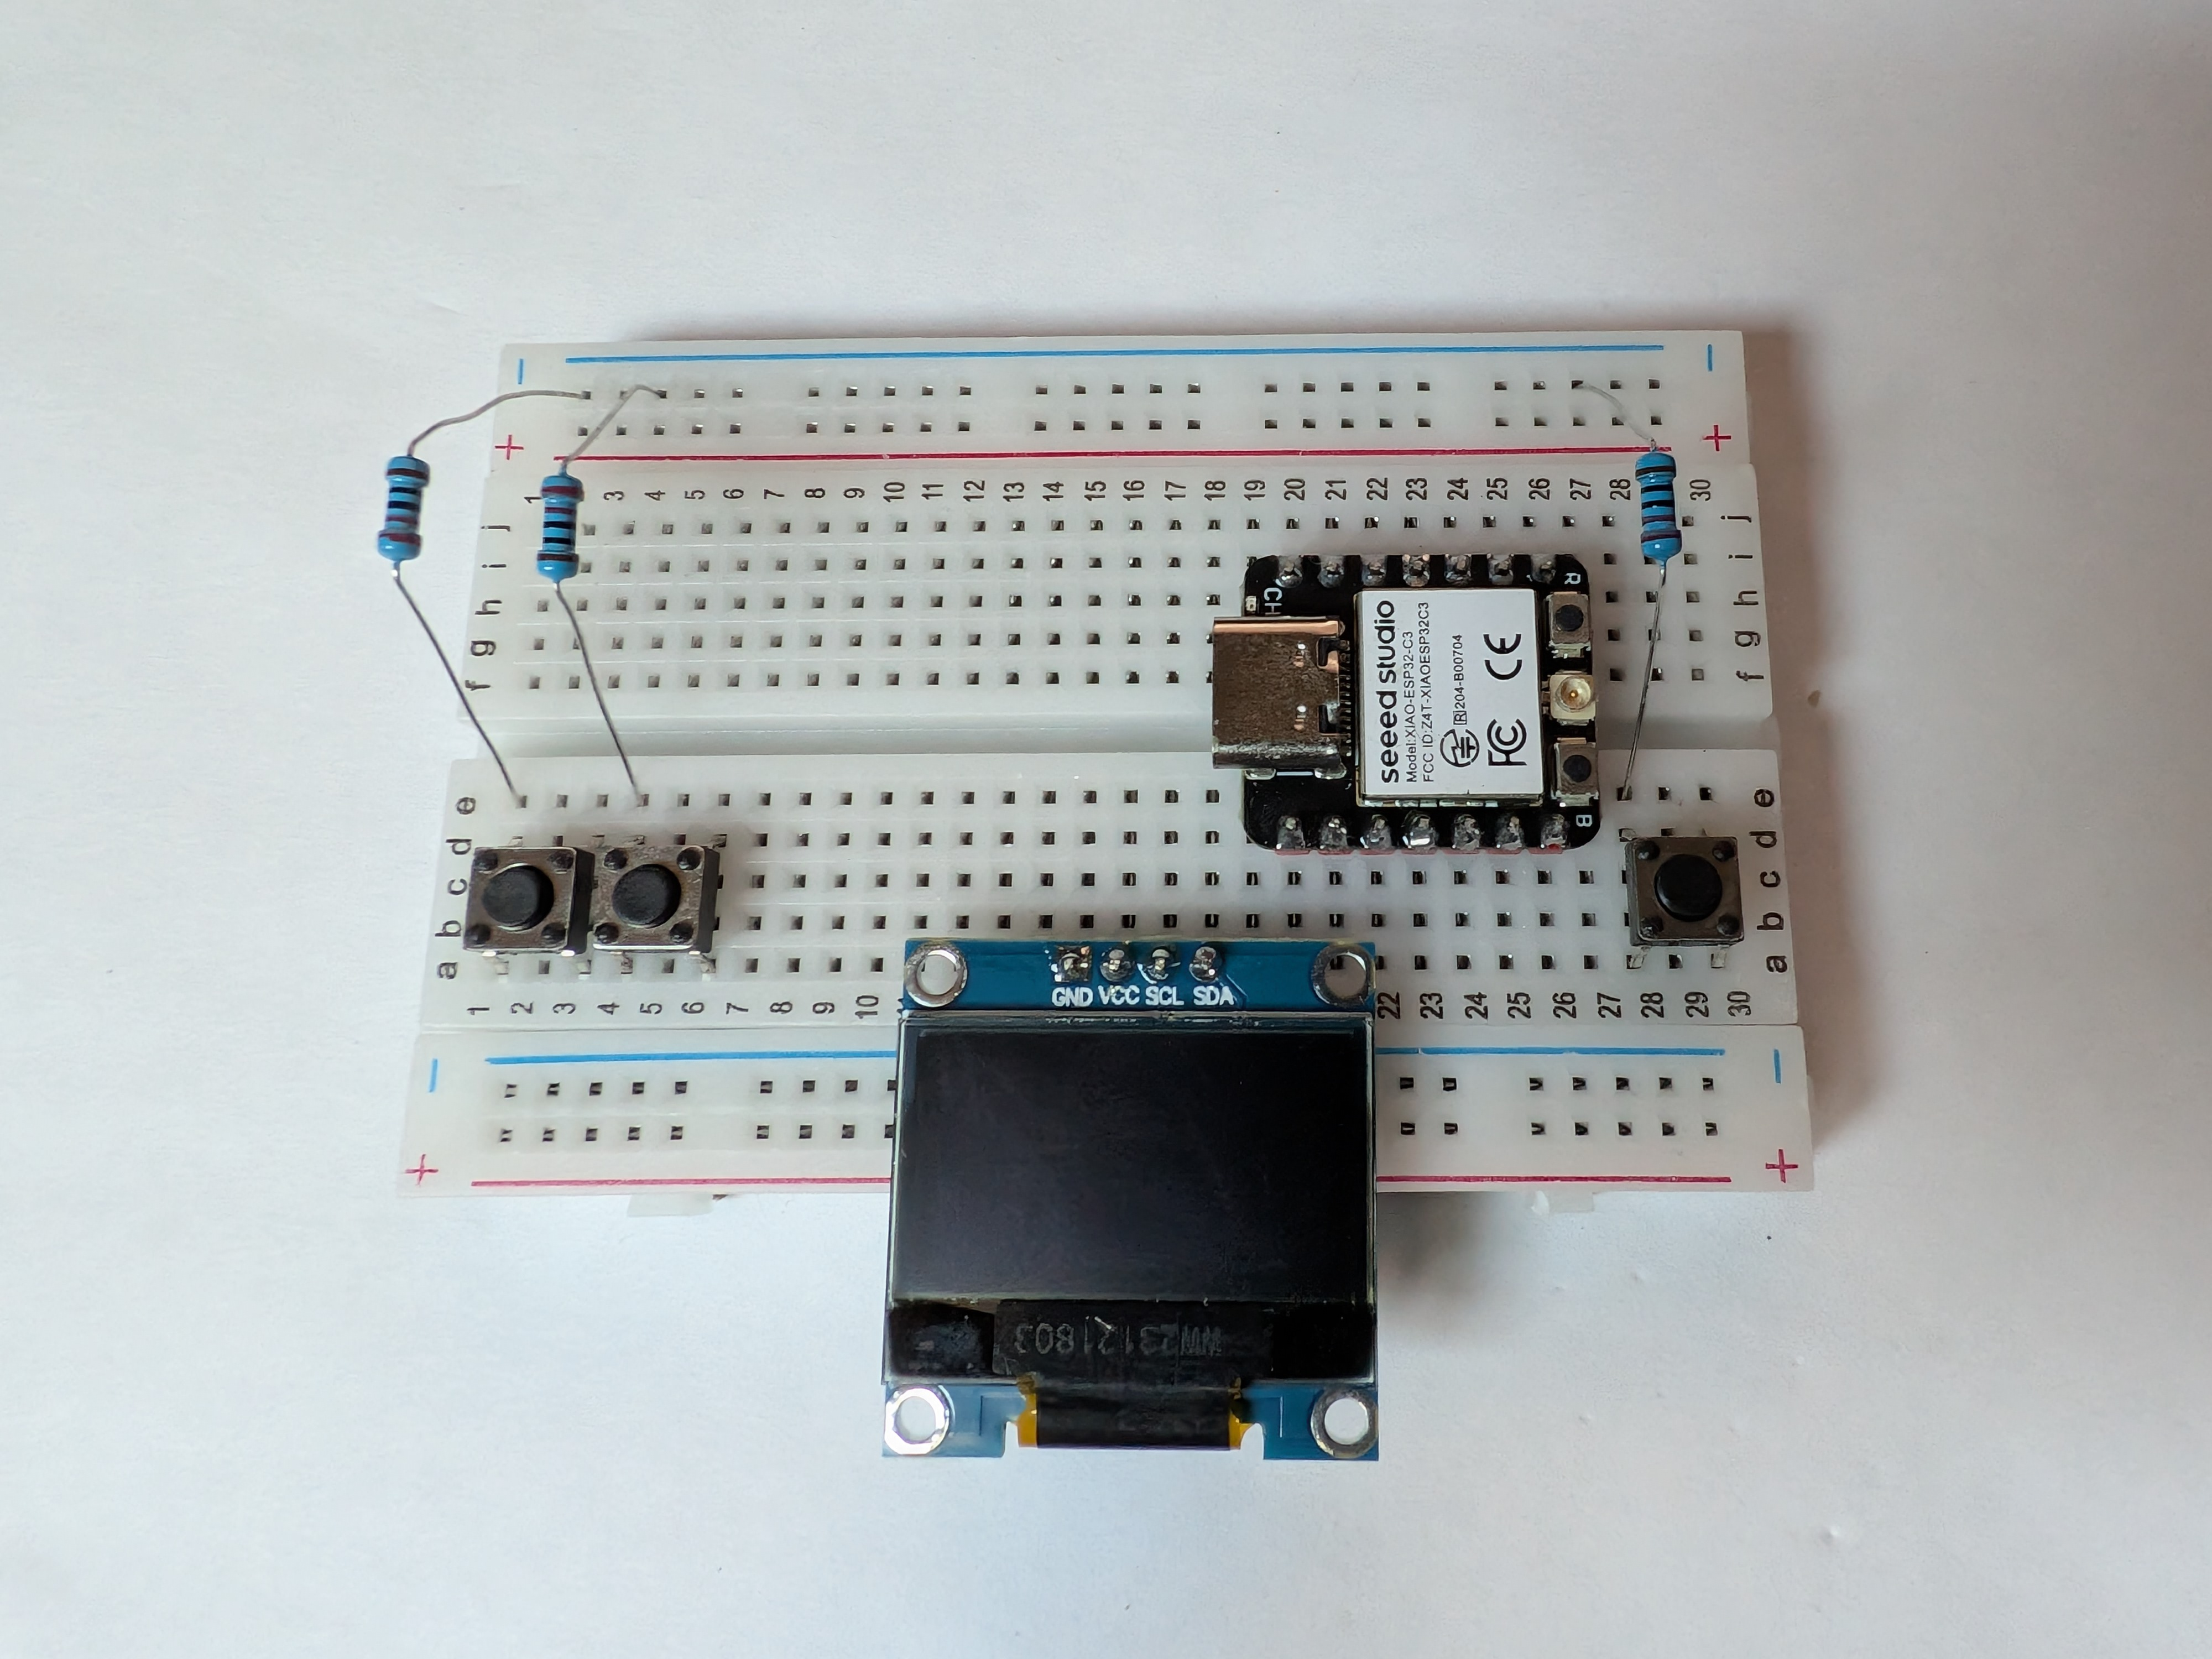
\includegraphics[width=.55\linewidth]{project_1/components_placed.jpg}
    \caption{All of the components except for the jumper wires are now placed.}
\end{figure}

\begin{tcolorbox}[colback=yellow!10!white,colframe=yellow!50!black]
    NOTE: Whenever you connect an LED to a microcontroller, you must always connect a resistor in series
    with it. In series means that the power goes in one leg of the LED, the other leg of the LED is attached
    to one leg of the resistor, and the ground completes the circuit from the other leg of the resistor.
    This is important so that you do not burn out the LED and/or the microcontroller pin.
\end{tcolorbox}

\subsubsection{Connect the necessary jumper wires}
\begin{itemize}
    \item Place one end of a red jumper wire into hole \textbf{J7} of the breadboard and the other end into
    \textbf{E16}. This will provide \textbf{3.3} volts of power to the LED when the program turns it on.
    \item Using a black jumper wire, place one end of the wire into hole \textbf{J2} of the breadboard and the other
    end into \textbf{E21}. This will provide a ground path for the LED through the resistor to complete the circuit.
\end{itemize}

You should be left with something that looks like this:
\begin{figure}[H]
    \centering
    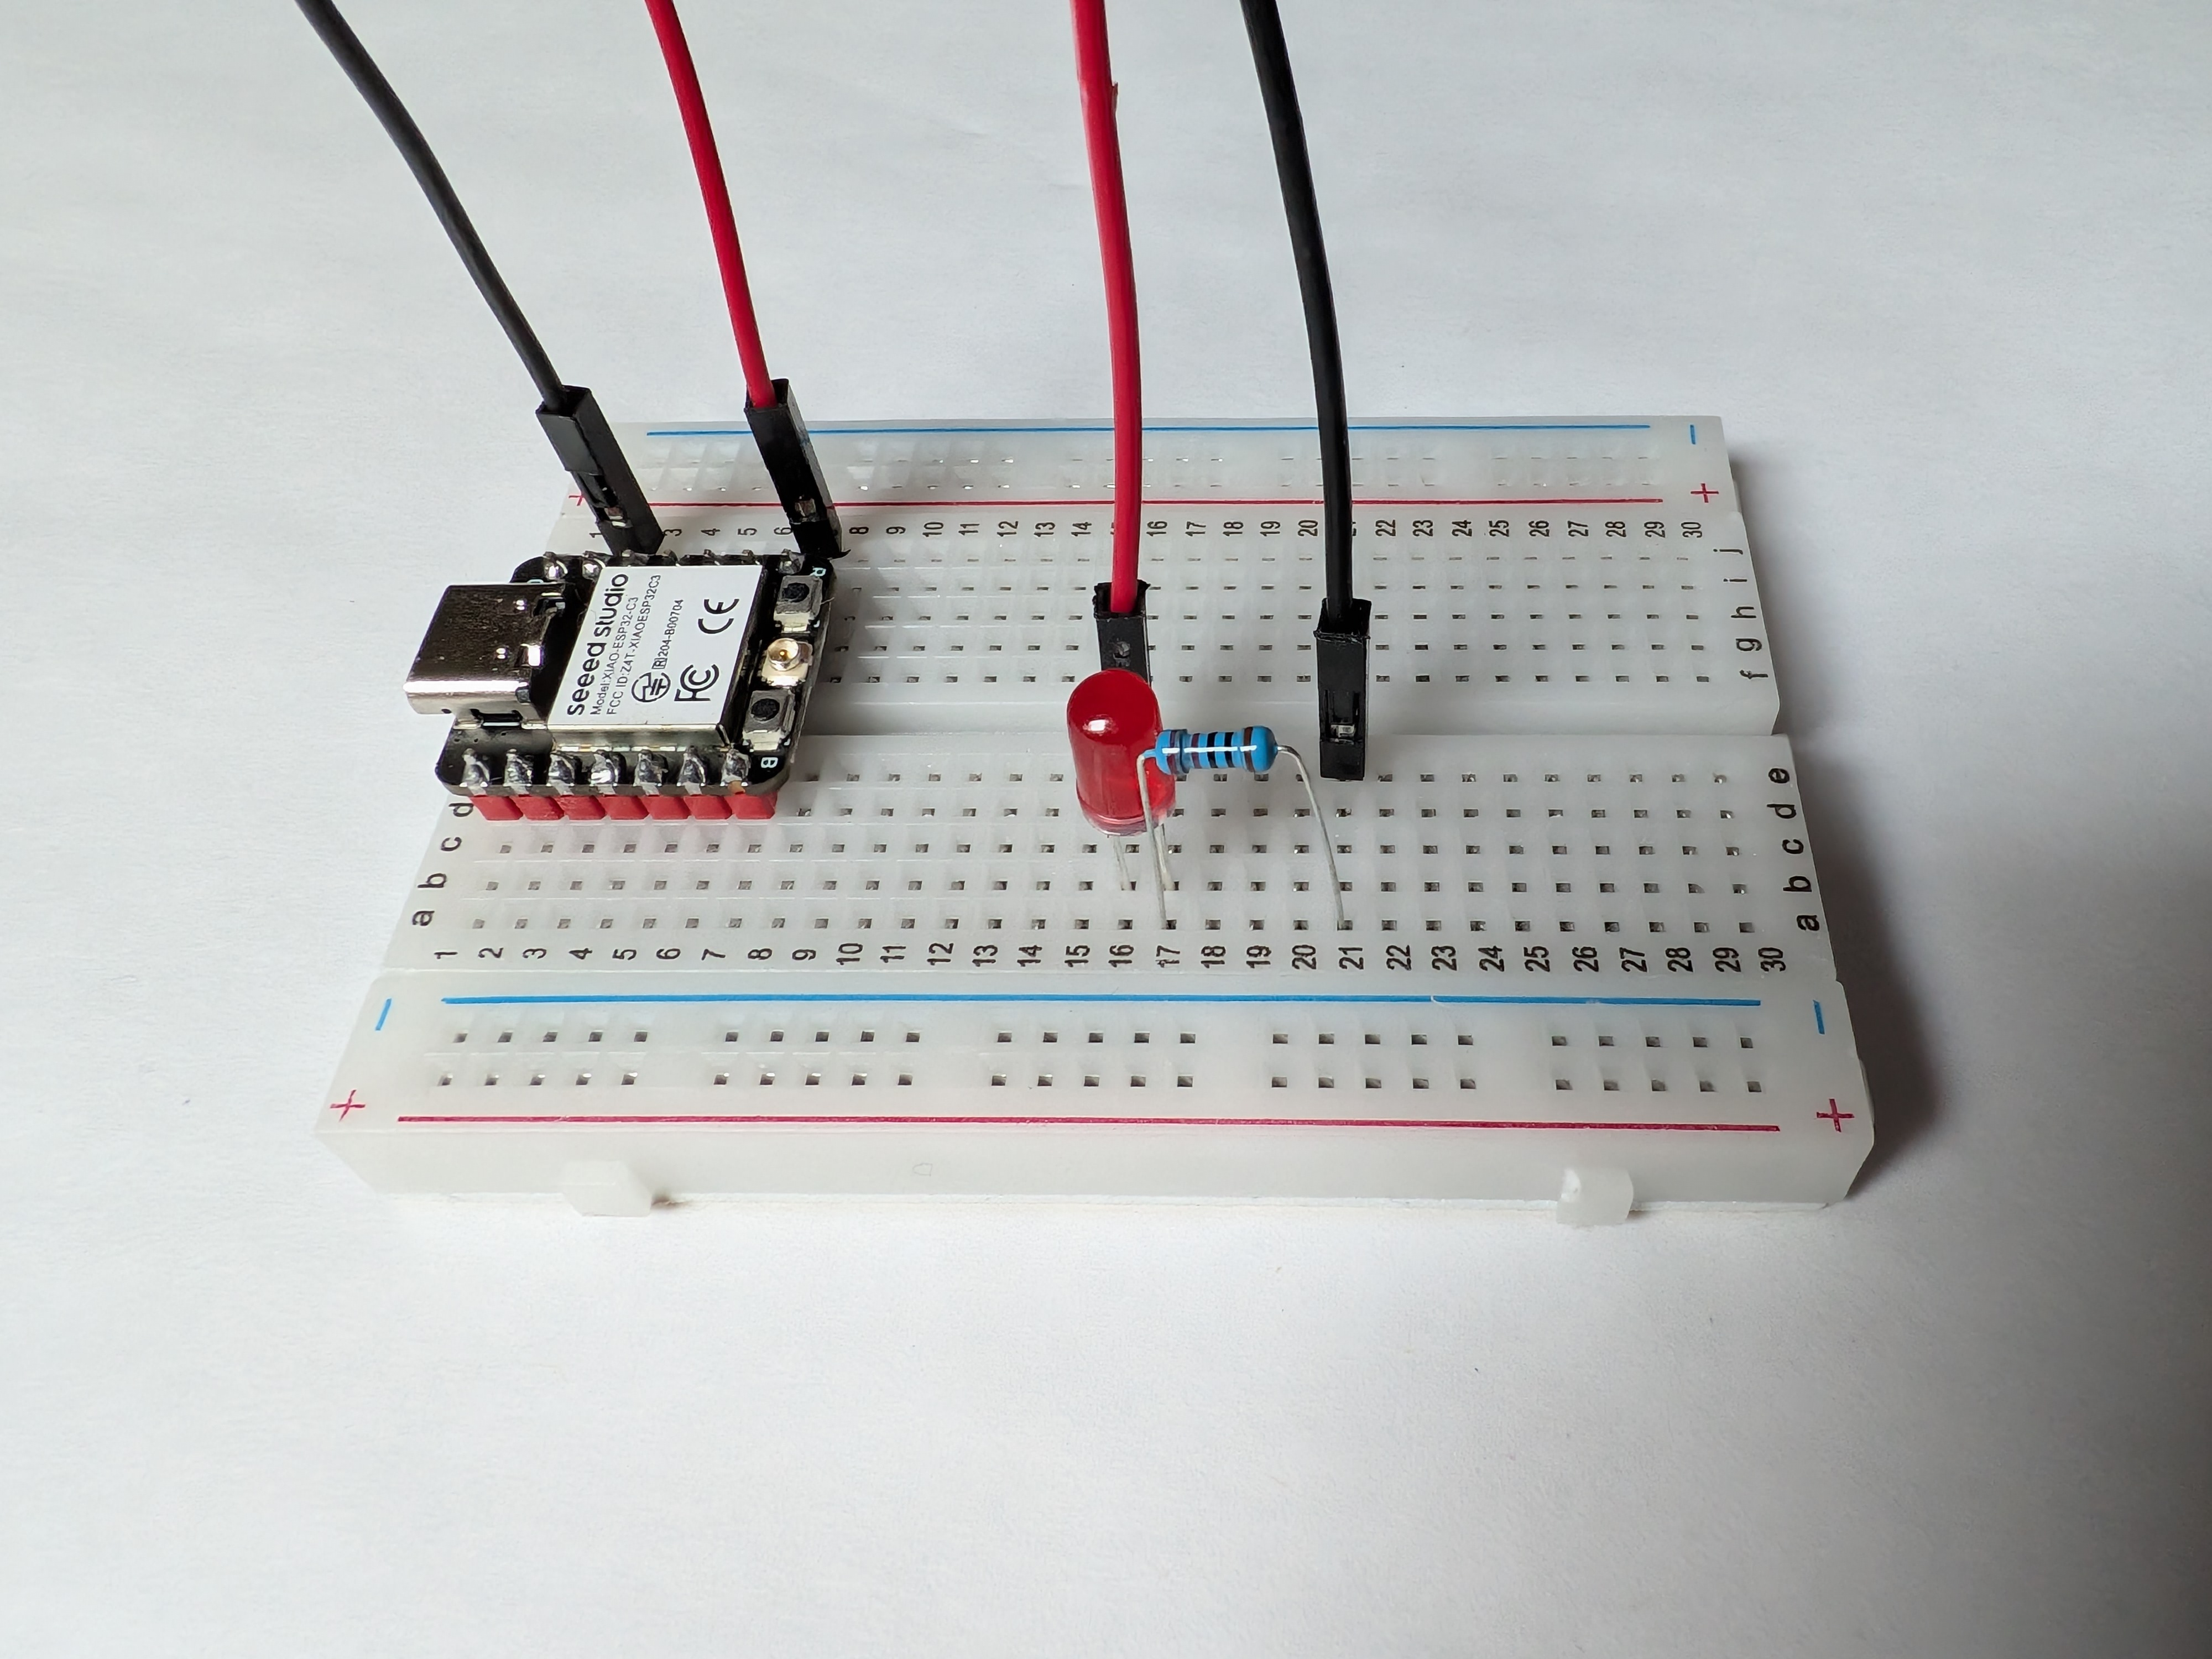
\includegraphics[width=.55\linewidth]{project_1/wired_up.jpg}
    \caption{I'm absolutely POSITIVE I connected everything correctly!}
\end{figure}

\subsection{Programming the microcontroller}

Once all of the wiring is correct, connect the USB cable to the microcontroller and load the IDE to
access it. Refer back to Chapter \ref{ide} for instructions.

Click on the file named "project\_1\_blink.py". This will load the code in the editor for this section.
Read through the comments and the code to get a sense for how it works. Once you are ready, you can
click the blue play button in the upper left of the window to start the script.

While the script is running, the LED will blink on and off waiting a half second inbetween each state.
You can stop the script by pressing the red stop button located where the blue play button used to be.

\section{Review}
In this project, we learned the basics of setting up a simple circuit and running some code to interact
with that circuit. We learned that some pins on the microcontroller can be programmed to turn connected
devices on and off. We also learned that connecting an LED in a circuit always requires adding a resistor
in series to prevent burning out the components.

\section{Possible Extensions}
If you want to do some experimentation, try these:

\begin{itemize}
    \item Update the code so that it sleeps for a random amount of time each loop
    \item Translate a message into morse code and have the LED blink out the message
\end{itemize}
